\section{Resultados}
Após Realizar o treinamento das 2 estruturas de redes propostas, as redes foram colocadas a prova a fim de avaliar seus resultados com os mesmos dados de treino validação e teste, conforme exposto na seção 3 sobre o banco de dados.

\subsection{Resultados MLP}
Depois de selecionado o número ideal para teste dessa estrutura de RNA, foi executado a resposta da rede tendo-se como base dados de teste das 3 classes do banco de dados.
\begin{figure}[H]
\centering % para centralizarmos a figura
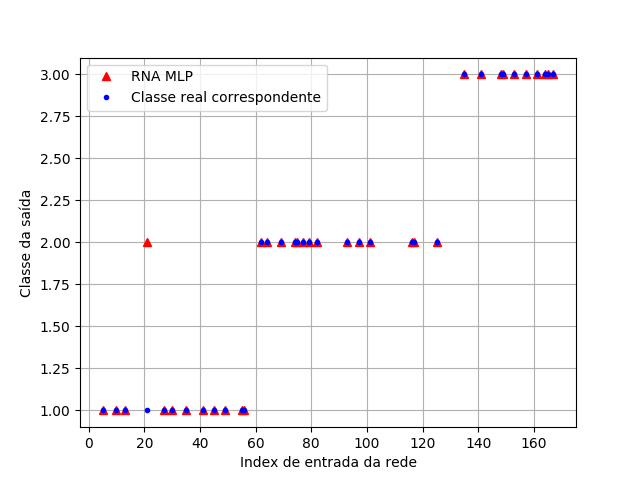
\includegraphics[width=\columnwidth]{04-Figuras/MLP}
\caption{Resposta da rede MLP}
\label{figura:acuracia}
\end{figure}
Realizado 10 repetições de treino validação e teste da rede com os mesmos dados, a percentagem de acerto da rede atingiu a marca de 95.27777778\%.
\subsection{Resultados RNA autoassociativa competitiva}
Feito a análise do melhor número de neurônios na camada escondida para a rede autoassociativa competitiva, cada RNA presente nessa estrutura apresentou um comportamento de erro quadrático médio diferente ao receber dados de teste das 3 classes de vinho presentes no banco de dados.
\begin{figure}[H]
\centering % para centralizarmos a figura
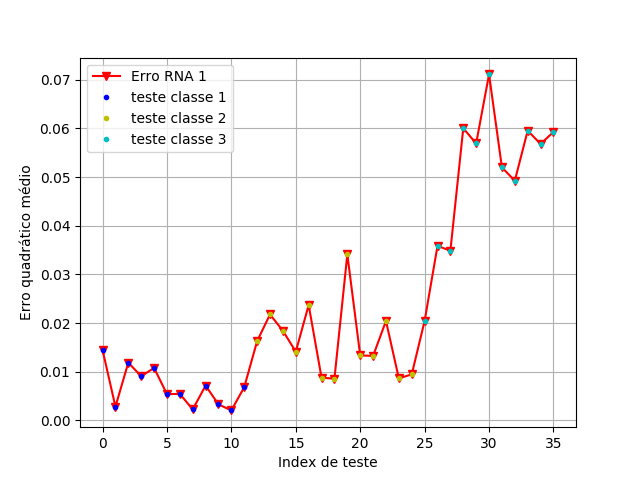
\includegraphics[width=\columnwidth]{04-Figuras/Erro_classe1_auto}
\caption{Erro da Rede 1 exposta os dados de treino}
\label{figura:acuracia}
\end{figure}
\begin{figure}[H]
\centering % para centralizarmos a figura
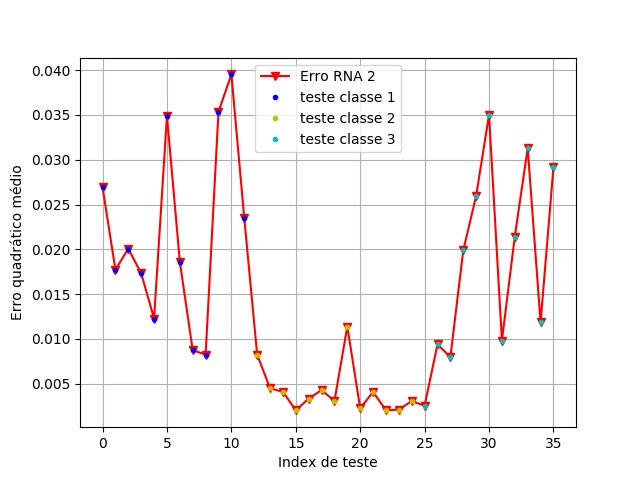
\includegraphics[width=\columnwidth]{04-Figuras/Erro_classe2_auto}
\caption{Erro da Rede 2 exposta os dados de treino}
\label{figura:acuracia}
\end{figure}
\begin{figure}[H]
\centering % para centralizarmos a figura
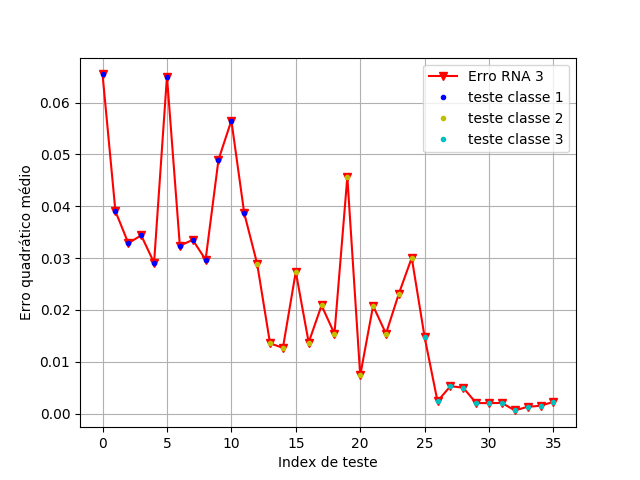
\includegraphics[width=\columnwidth]{04-Figuras/Erro_classe3_auto}
\caption{Erro da Rede 3 exposta os dados de treino}
\label{figura:acuracia}
\end{figure}
Nota-se que a Rede 1, Rede 2 e Rede 3 foram treinadas com bases de dados respectivamente da classe 1,2 e 3.

A saída dessa estrutura de rede se beneficiou do comportamento do erro quadrático médio demonstrado acima, apresentando uma marca de 100\% de acerto médio em 10 repetições de treino validação e teste,  utilizando os mesmos dados de entrada.
\begin{figure}[H]
\centering % para centralizarmos a figura
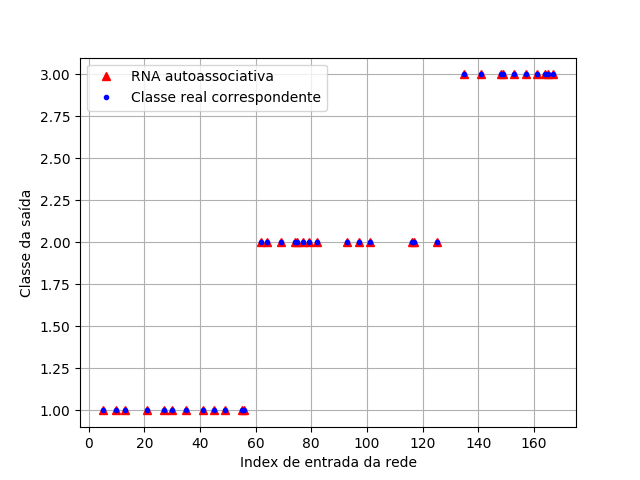
\includegraphics[width=\columnwidth]{04-Figuras/auto_mlp_out}
\caption{Saída da Rede Autoassociativa Competitiva}

\label{figura:acuracia}
\end{figure}

\subsection{Comparativo do desempenho}
Após realizados os testes de desempenho das 2 estruturas,o comparativo de desempenho de ambas foi disposto na Tabela 4.
\begin{table}[H]
\centering
\caption{Comparativo de Desempenho}
\resizebox{\columnwidth}{!}{%
\begin{tabular}{cccc}
\hline
Estrutura da RNA & \begin{tabular}[c]{@{}c@{}}Acurácia média \% \\ \\ de 10 repetições\end{tabular} & Tempo de execução(s) & \begin{tabular}[c]{@{}c@{}}Nº de Épocas\\ \\ utilizadas\\  no treinamento\end{tabular} \\ \hline
MLP & 95.277778 & 3.908075 & 400 \\
\begin{tabular}[c]{@{}c@{}}Autoassociativa \\ \\ competitiva\end{tabular} & 100 & 8.684611 & \begin{tabular}[c]{@{}c@{}}3000 p/ \\ \\ cada rede\end{tabular} \\ \hline
\end{tabular}
}
\label{tabela:baseDados}

\end{table}


Com base nos dados dispostos na Tabela 4, é possível afirmar que a Rede autoassociativa apresentou a marca impecável de 100\% de acerto, devido ao comportamento das redes associadas, de forma que cada rede treinada com dados de apenas 1 classe desempenhava um papel de filtro com relação aos dados das outras classes. De forma que uma rede autoencoder que foi treinada apenas com dados de 1 classe apresentava erro quadrático médio menor quando comparado-se com as outras redes, assim, quando realizado a competição entre as 3 redes treinadas, a classe de saída era escolhida com uma maior acurácia quando comparado-se com o processo de escolha da de apenas uma MLP.